\def\layersep{1.3cm}
\def\outsep{0.5cm}
\def\dy{0.7}

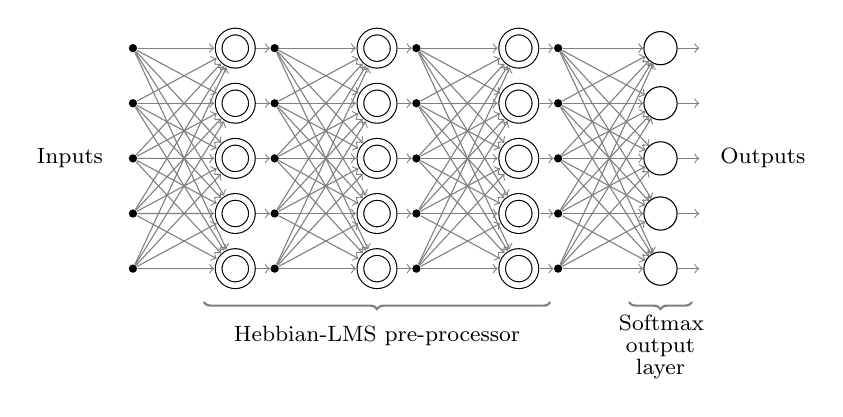
\begin{tikzpicture}[->, shorten >= 0pt, draw=black!50, node distance=\layersep,font=\fontsize{8}{8}\selectfont]
    \tikzstyle{node}=[circle,fill=black,minimum size=3pt,inner sep=0pt]
    \tikzstyle{nothing}=[draw=none,minimum size=0pt,inner sep=0pt]
    \tikzstyle{neuron}=[draw=black,circle,fill=none,minimum size=12pt,inner sep=0pt]
    \tikzstyle{HLMS neuron}=[neuron, double, double distance=2pt]

	%%%% Layer 1
    \foreach \name / \y in {1,...,5} {
    % This is the same as writing \foreach \name / \y in {1/1,2/2,3/3,4/4}
        \node[node] (I1-\name) at (0,-\dy*\y) {}; % Draw the input layer nodes
        \node[HLMS neuron] (H1-\name) at (\layersep,-\dy*\y cm) {}; % Draw the hidden layer nodes
        \node[node] (O1-\name) at (\layersep+\outsep,-\dy*\y cm) {}; % Draw the output layer node     
        \draw[->,shorten >=0cm,shorten <=0.05cm] (H1-\name) -- (O1-\name);
     }   	
    % Connect every node in the input layer with every node in the
    % hidden layer.
    \foreach \source in {1,...,5}
        \foreach \dest in {1,...,5}
            \draw[->,shorten >=0.05cm,shorten <=0cm] (I1-\source) -> (H1-\dest);

	%%%% Layer 2
    \foreach \name / \y in {1,...,5} {
    % This is the same as writing \foreach \name / \y in {1/1,2/2,3/3,4/4}
        \node[HLMS neuron] (H2-\name) at (2*\layersep+\outsep,-\dy*\y cm) {}; % Draw the hidden layer nodes
        \node[node] (O2-\name) at (2*\layersep+2*\outsep,-\dy*\y cm) {}; % Draw the output layer node
        \draw[->,shorten >=0cm,shorten <=0.05cm] (H2-\name) -- (O2-\name);
     }   	
    % Connect every node in the input layer with every node in the
    % hidden layer.
    \foreach \source in {1,...,5}
        \foreach \dest in {1,...,5}
            \draw[->,shorten >=0.05cm,shorten <=0cm] (O1-\source) edge (H2-\dest);
    
    %%%% Layer 3
    \foreach \name / \y in {1,...,5} {
    % This is the same as writing \foreach \name / \y in {1/1,2/2,3/3,4/4}
        \node[HLMS neuron] (H3-\name) at (3*\layersep+2*\outsep,-\dy*\y cm) {}; % Draw the hidden layer nodes
        \node[node] (O3-\name) at (3*\layersep+3*\outsep,-\dy*\y cm) {}; % Draw the output layer node
        \draw[->,shorten >=0cm,shorten <=0.05cm] (H3-\name) -- (O3-\name);
     }   	
    % Connect every node in the input layer with every node in the
    % hidden layer.
    \foreach \source in {1,...,5}
        \foreach \dest in {1,...,5}
            \draw[->,shorten >=0.05cm,shorten <=0cm] (O2-\source) edge (H3-\dest);
        
    %%%% Layer 4
    \foreach \name / \y in {1,...,5} {
    % This is the same as writing \foreach \name / \y in {1/1,2/2,3/3,4/4}
        \node[neuron] (H4-\name) at (4*\layersep+3*\outsep,-\dy*\y cm) {}; % Draw the hidden layer nodes
        \node[nothing] (O4-\name) at (4*\layersep+4*\outsep,-\dy*\y cm) {}; % Draw the output layer node
        \path (H4-\name) edge (O4-\name);
     }   	
    % Connect every node in the input layer with every node in the
    % hidden layer.
    \foreach \source in {1,...,5}
        \foreach \dest in {1,...,5} 
            \draw (O3-\source) edge (H4-\dest);

	%% Text
    \node[left of=I1-3, node distance=0.8cm] (in) {Inputs};
    \node[right of=O4-3, node distance=0.8cm] (out) {Outputs};
	\draw[-,decoration={brace,mirror,raise=5pt},decorate, thick]
   (0.9, -3.75) -- node[below=10pt] {Hebbian-LMS pre-processor} (5.3, -3.75);
   \draw[-,decoration={brace,mirror,raise=5pt},decorate, thick, text width=3em, text centered]
   (6.3, -3.75) -- node[below=6pt] {Softmax output layer} (7.1, -3.75);
\end{tikzpicture}